\appendix{Представление графического материала}

Графический материал, выполненный на отдельных листах,
изображен на рисунках А.1 - А.9.

\setcounter{числоПлакатов}{0}
\renewcommand{\thefigure}{А.\arabic{figure}} % шаблон номера для плакатов

\begin{landscape}
	\setcounter{page}{74}
	\begin{плакат}
		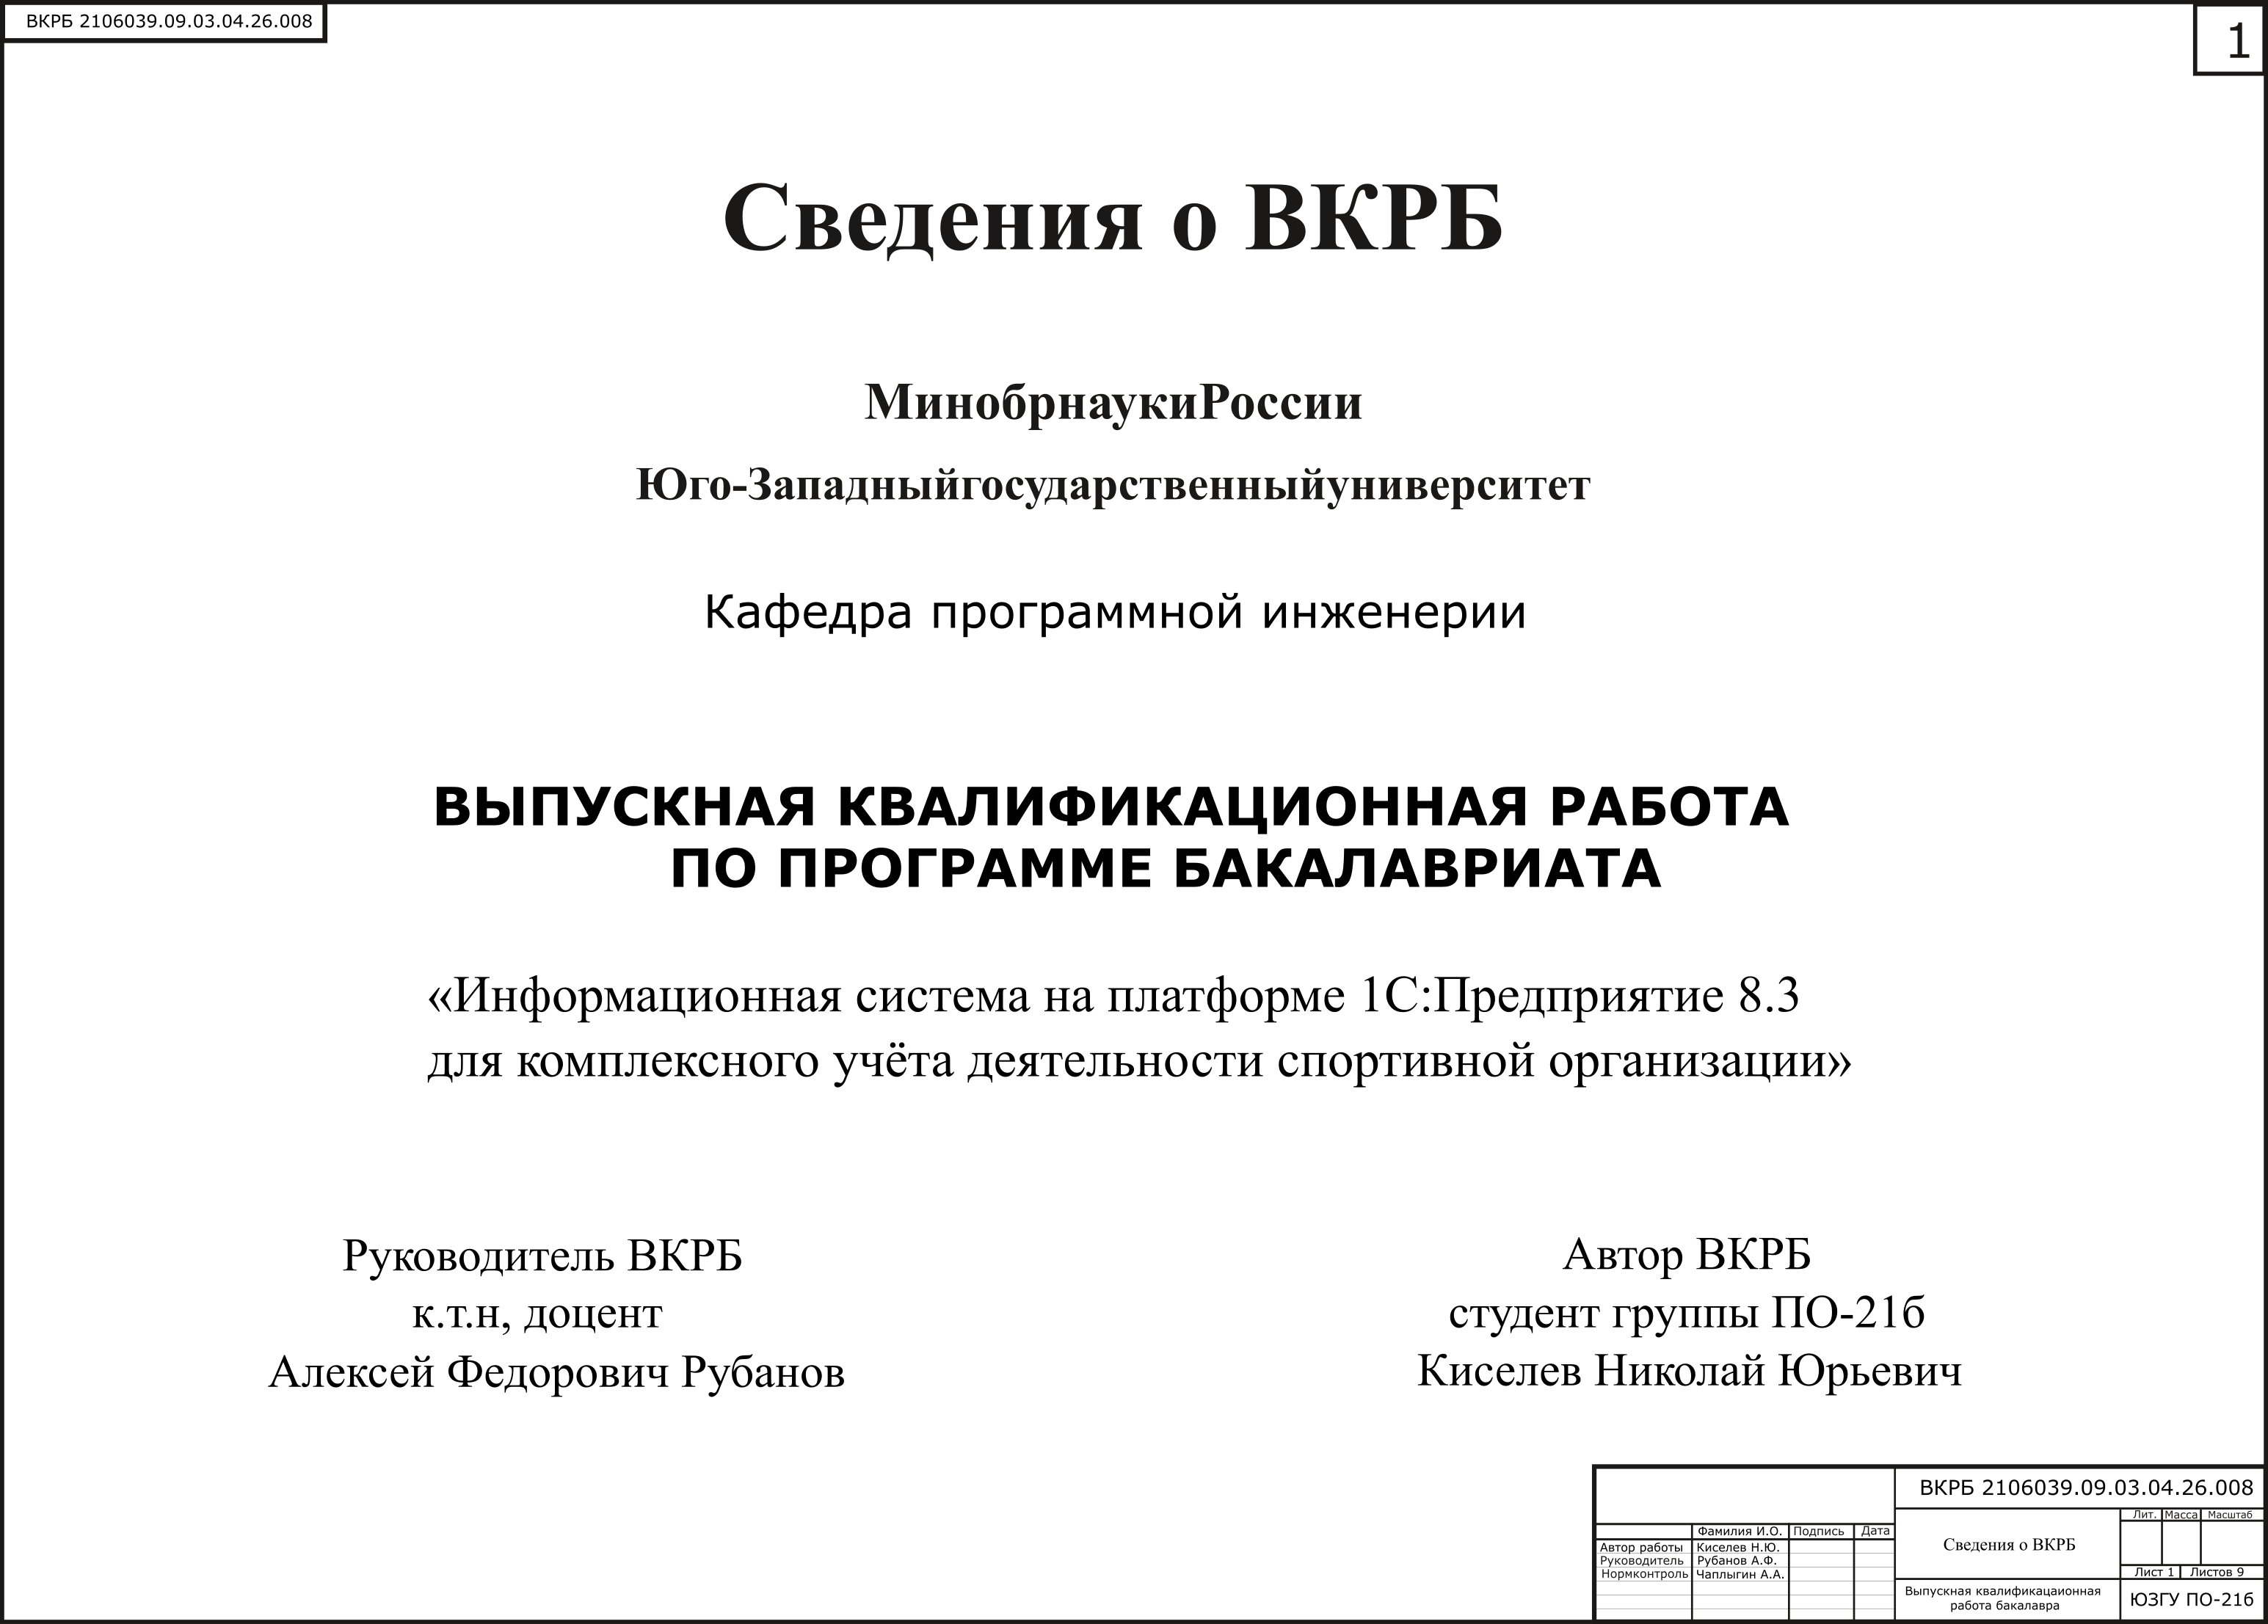
\includegraphics[width=0.85\linewidth]{images/Diplom1.png}
		\заголовок{Сведения о ВКРБ}
		\label{pl1:image}
	\end{плакат}
	
	
	\begin{плакат}
		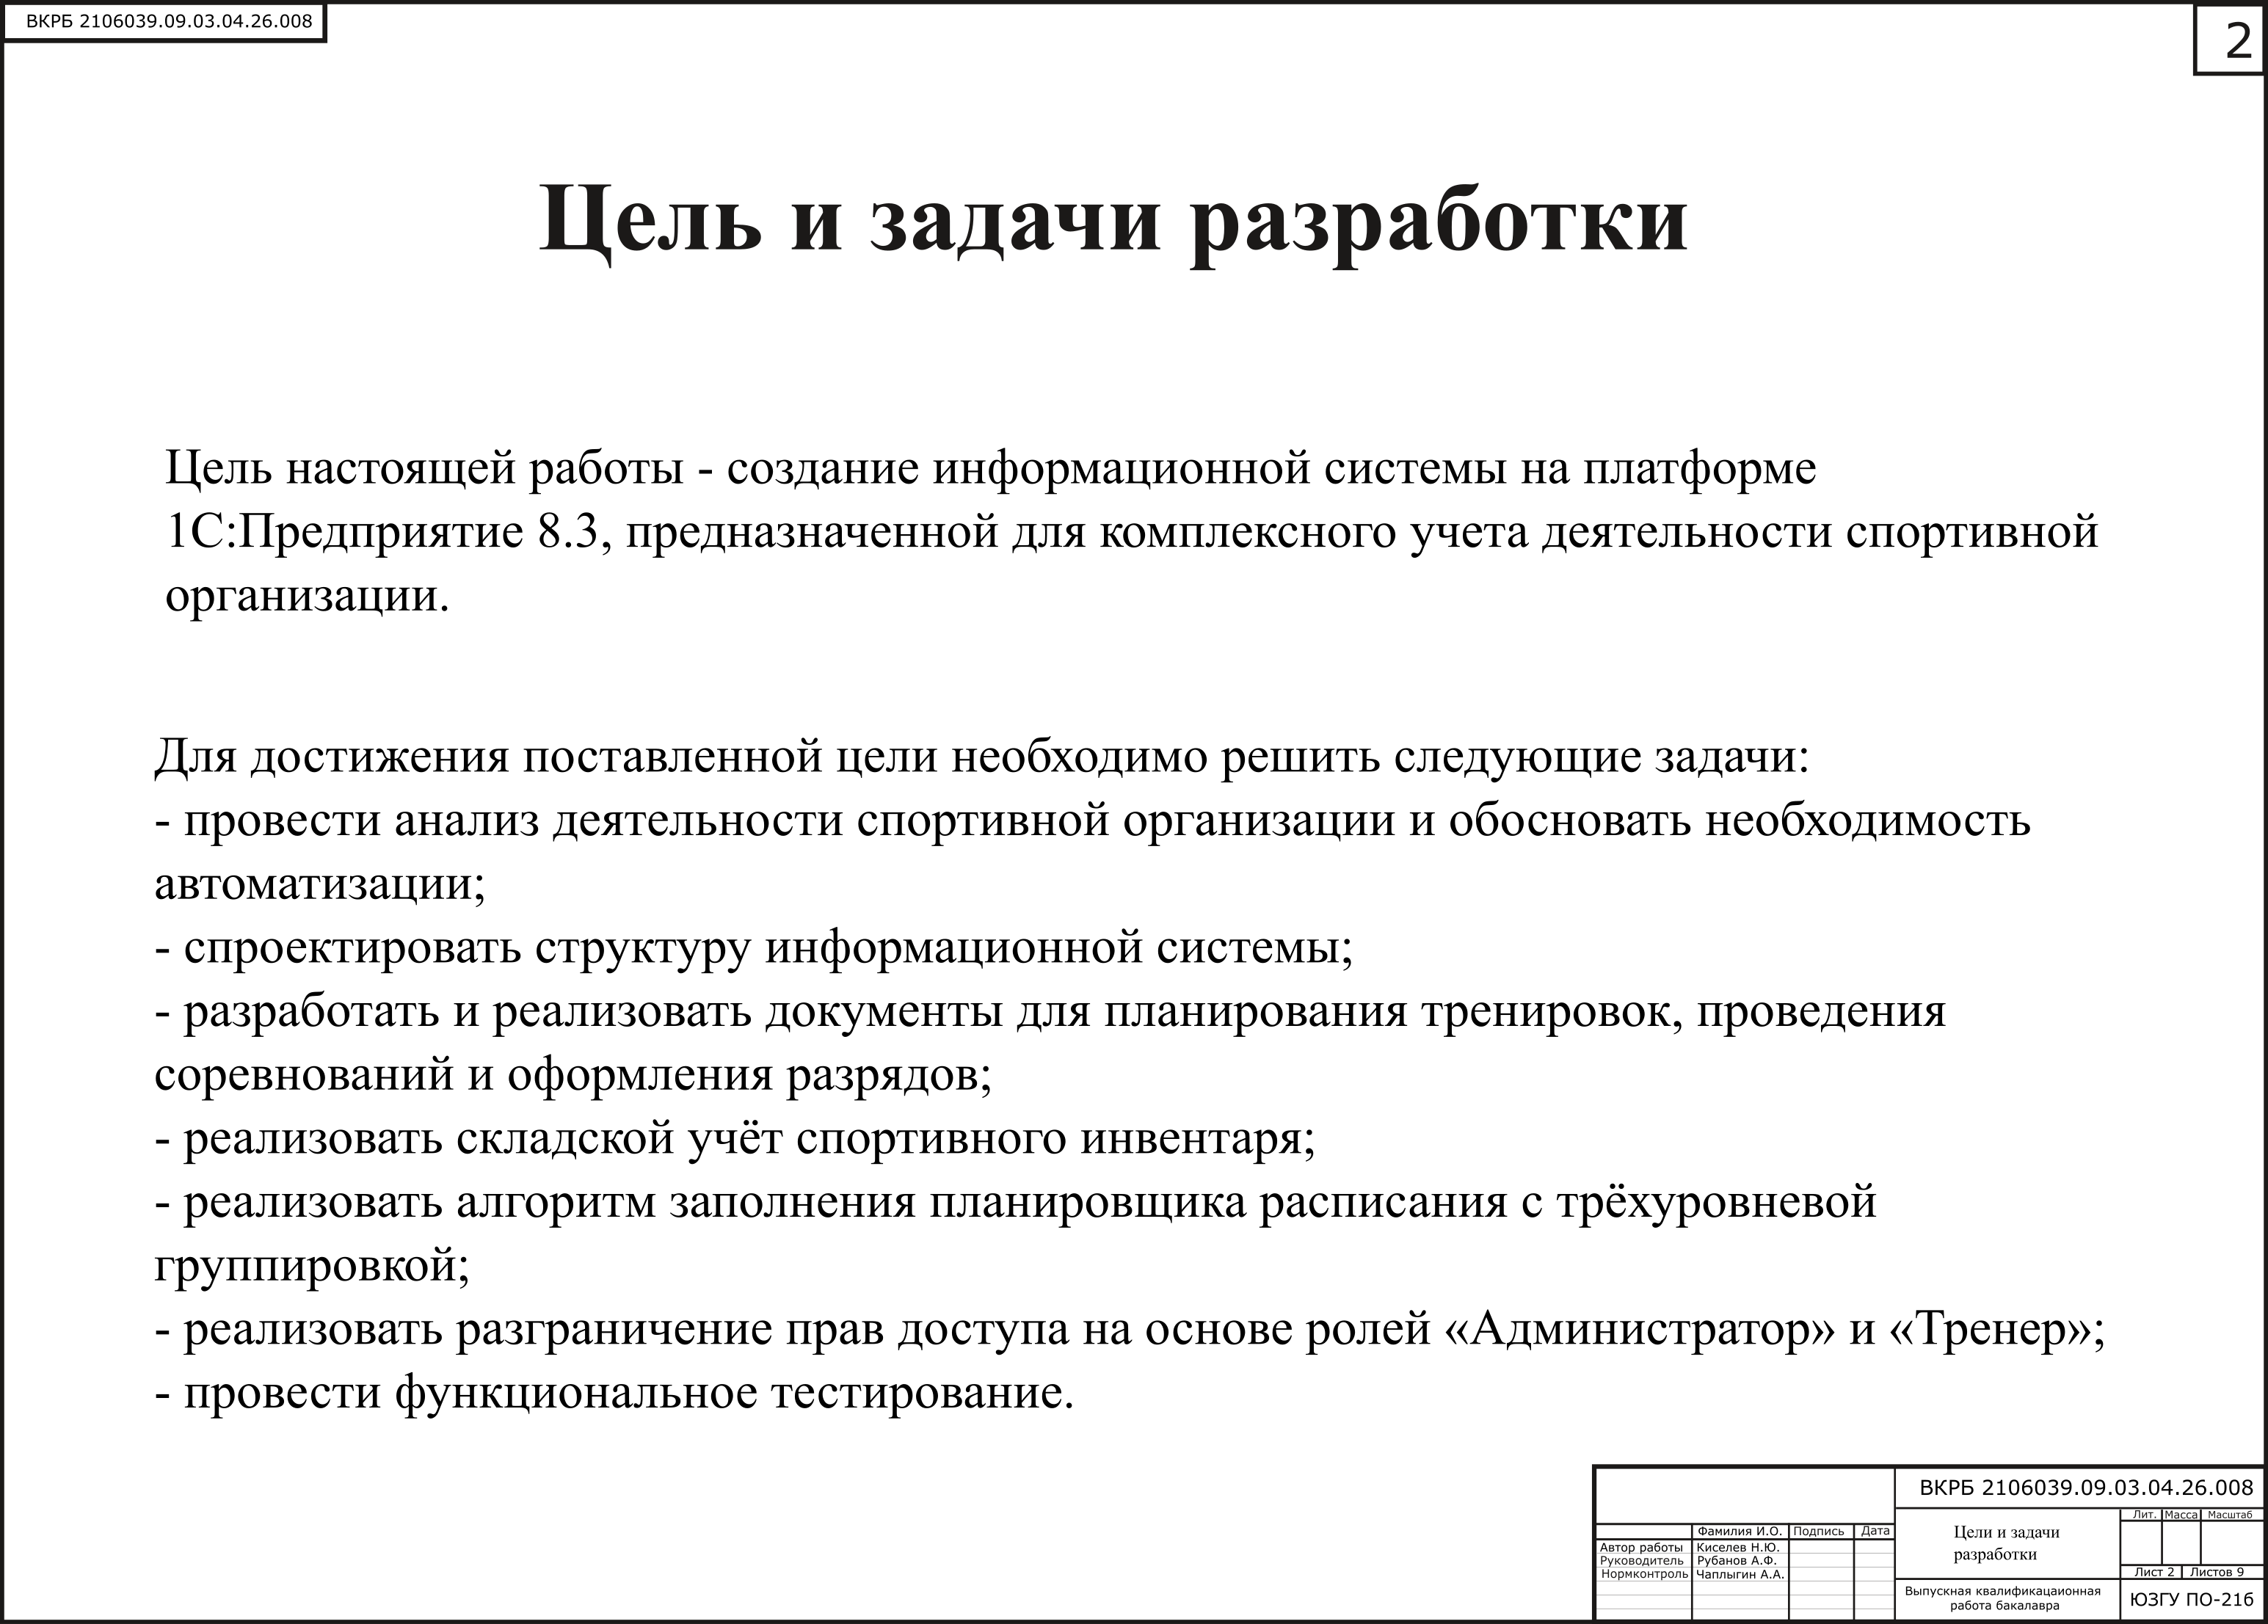
\includegraphics[width=0.85\linewidth]{images/Diplom2.png}
		\заголовок{Цель и задачи разработки}
		\label{pl2:image}      
	\end{плакат}
	
	\begin{плакат}
		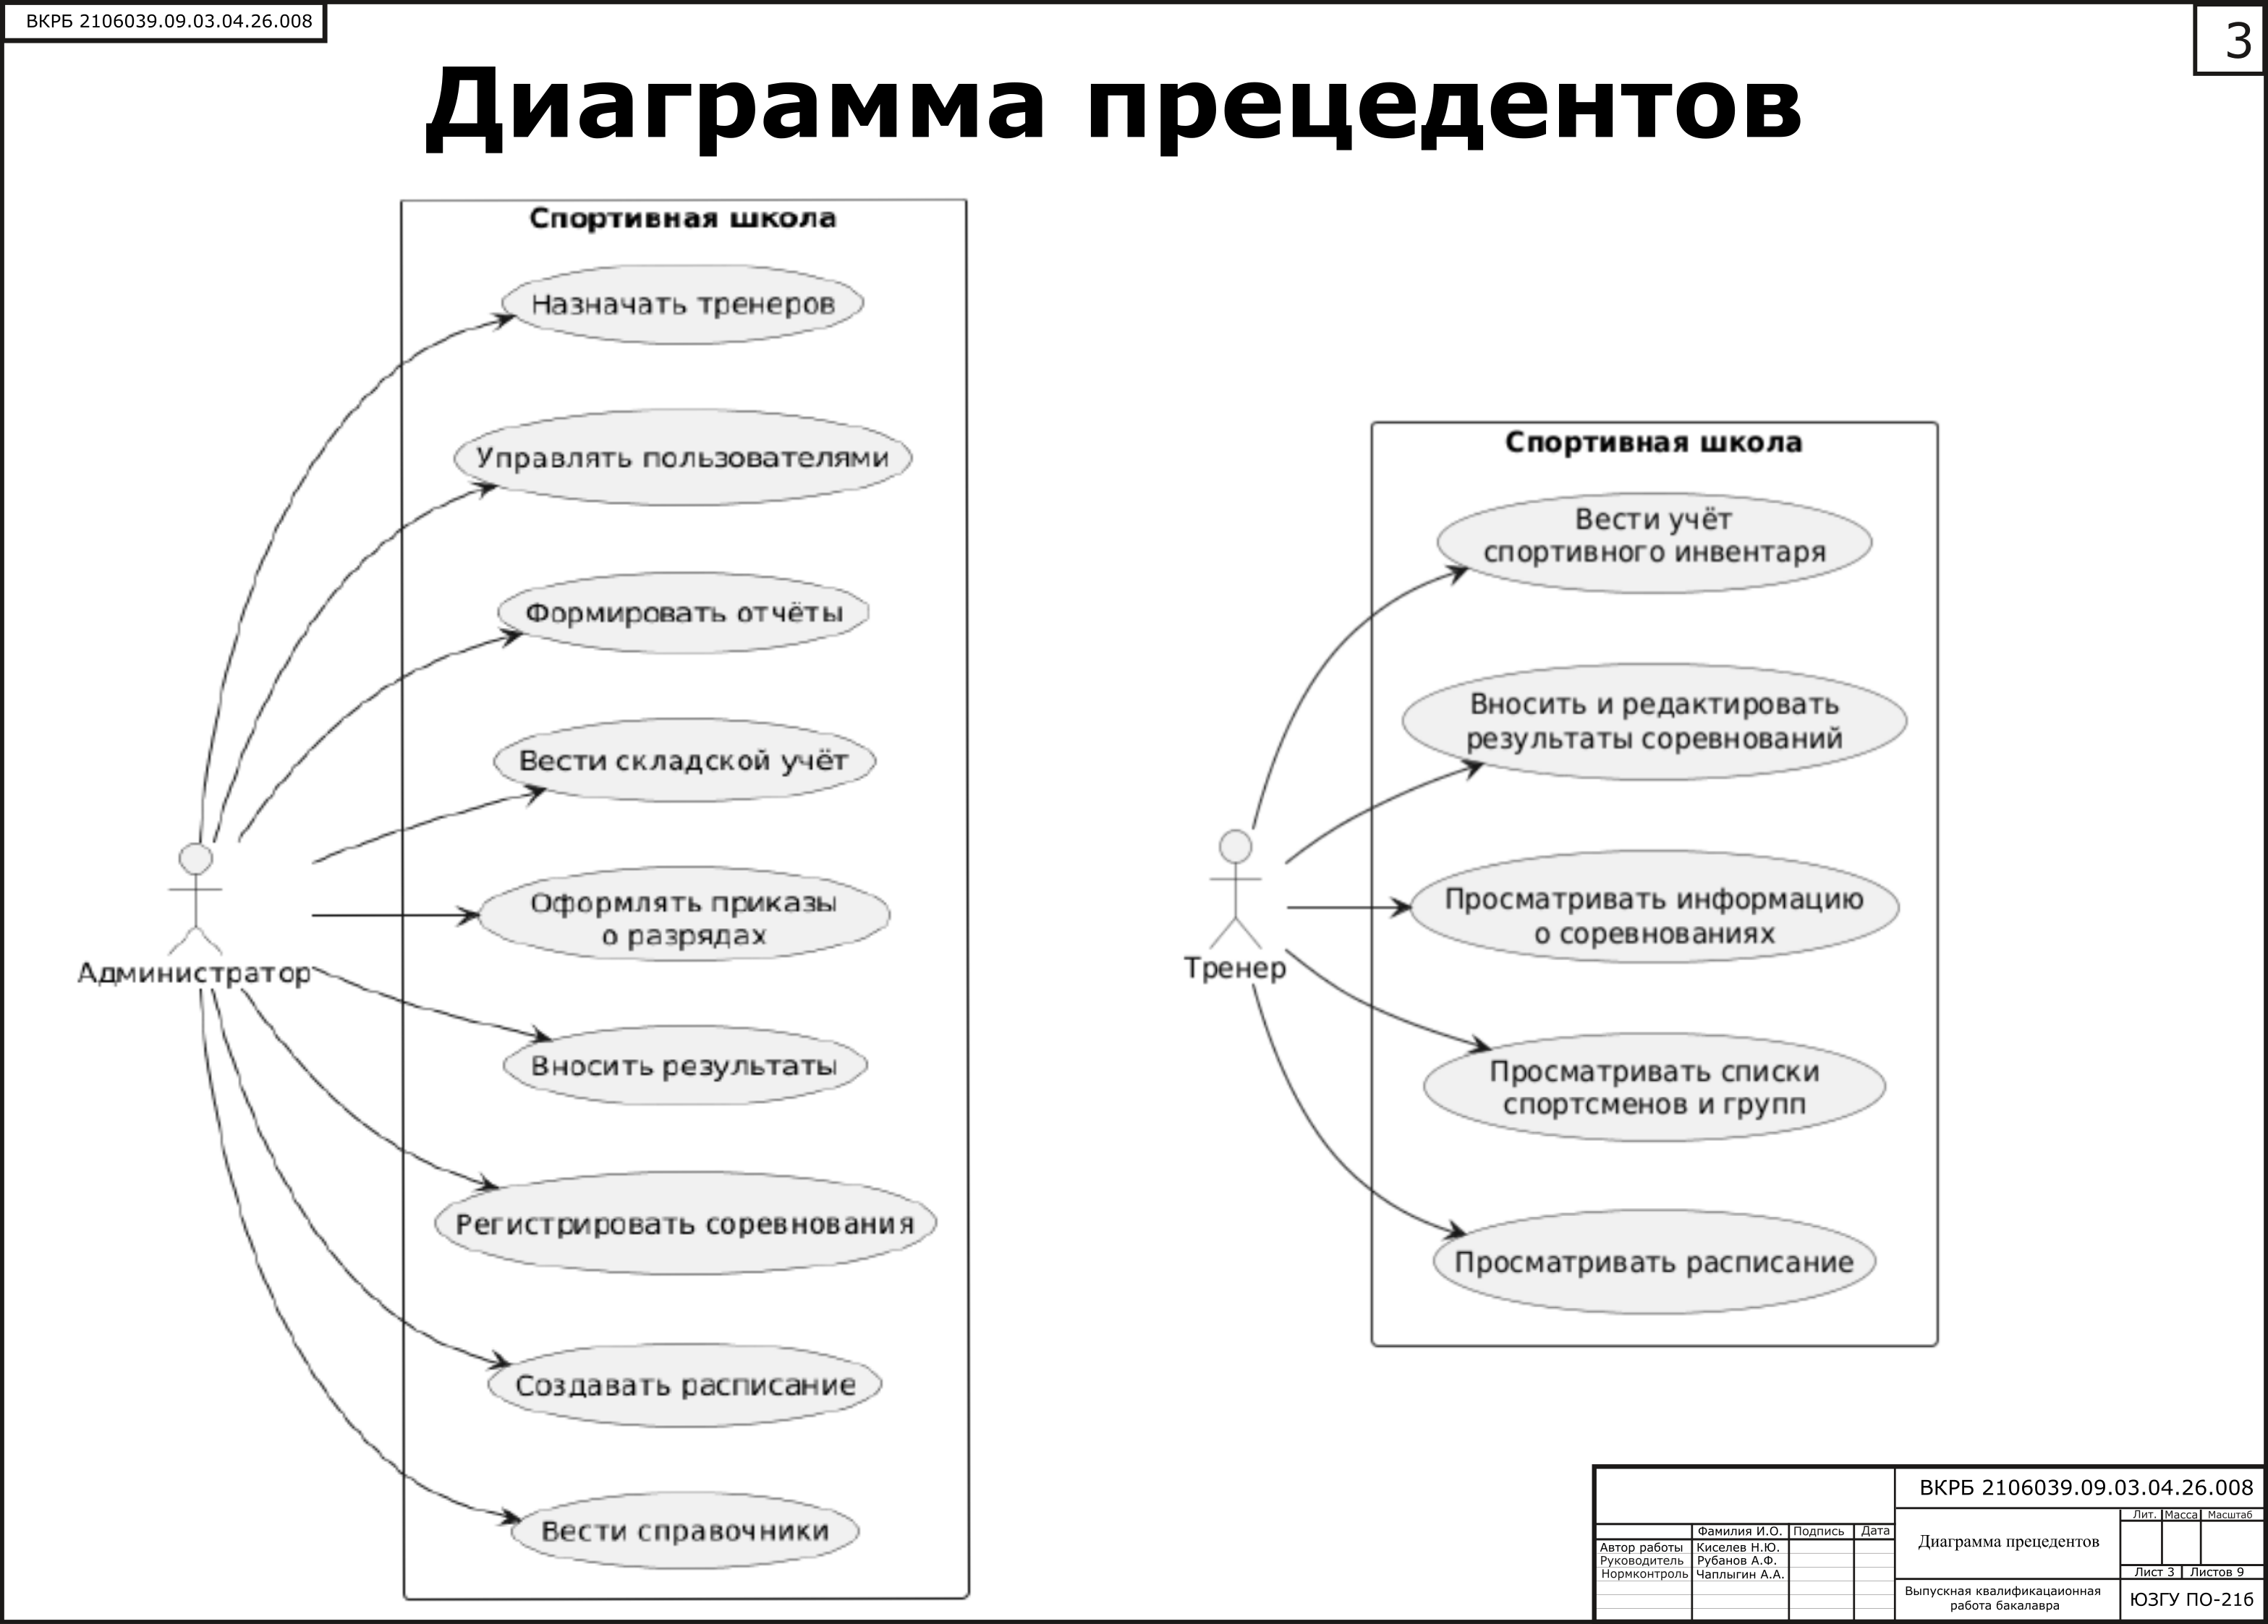
\includegraphics[width=0.85\linewidth]{images/Diplom3.png}
		\заголовок{Диаграмма прецедентов}
		\label{pl3:image}      
	\end{плакат}
	
	\begin{плакат}
		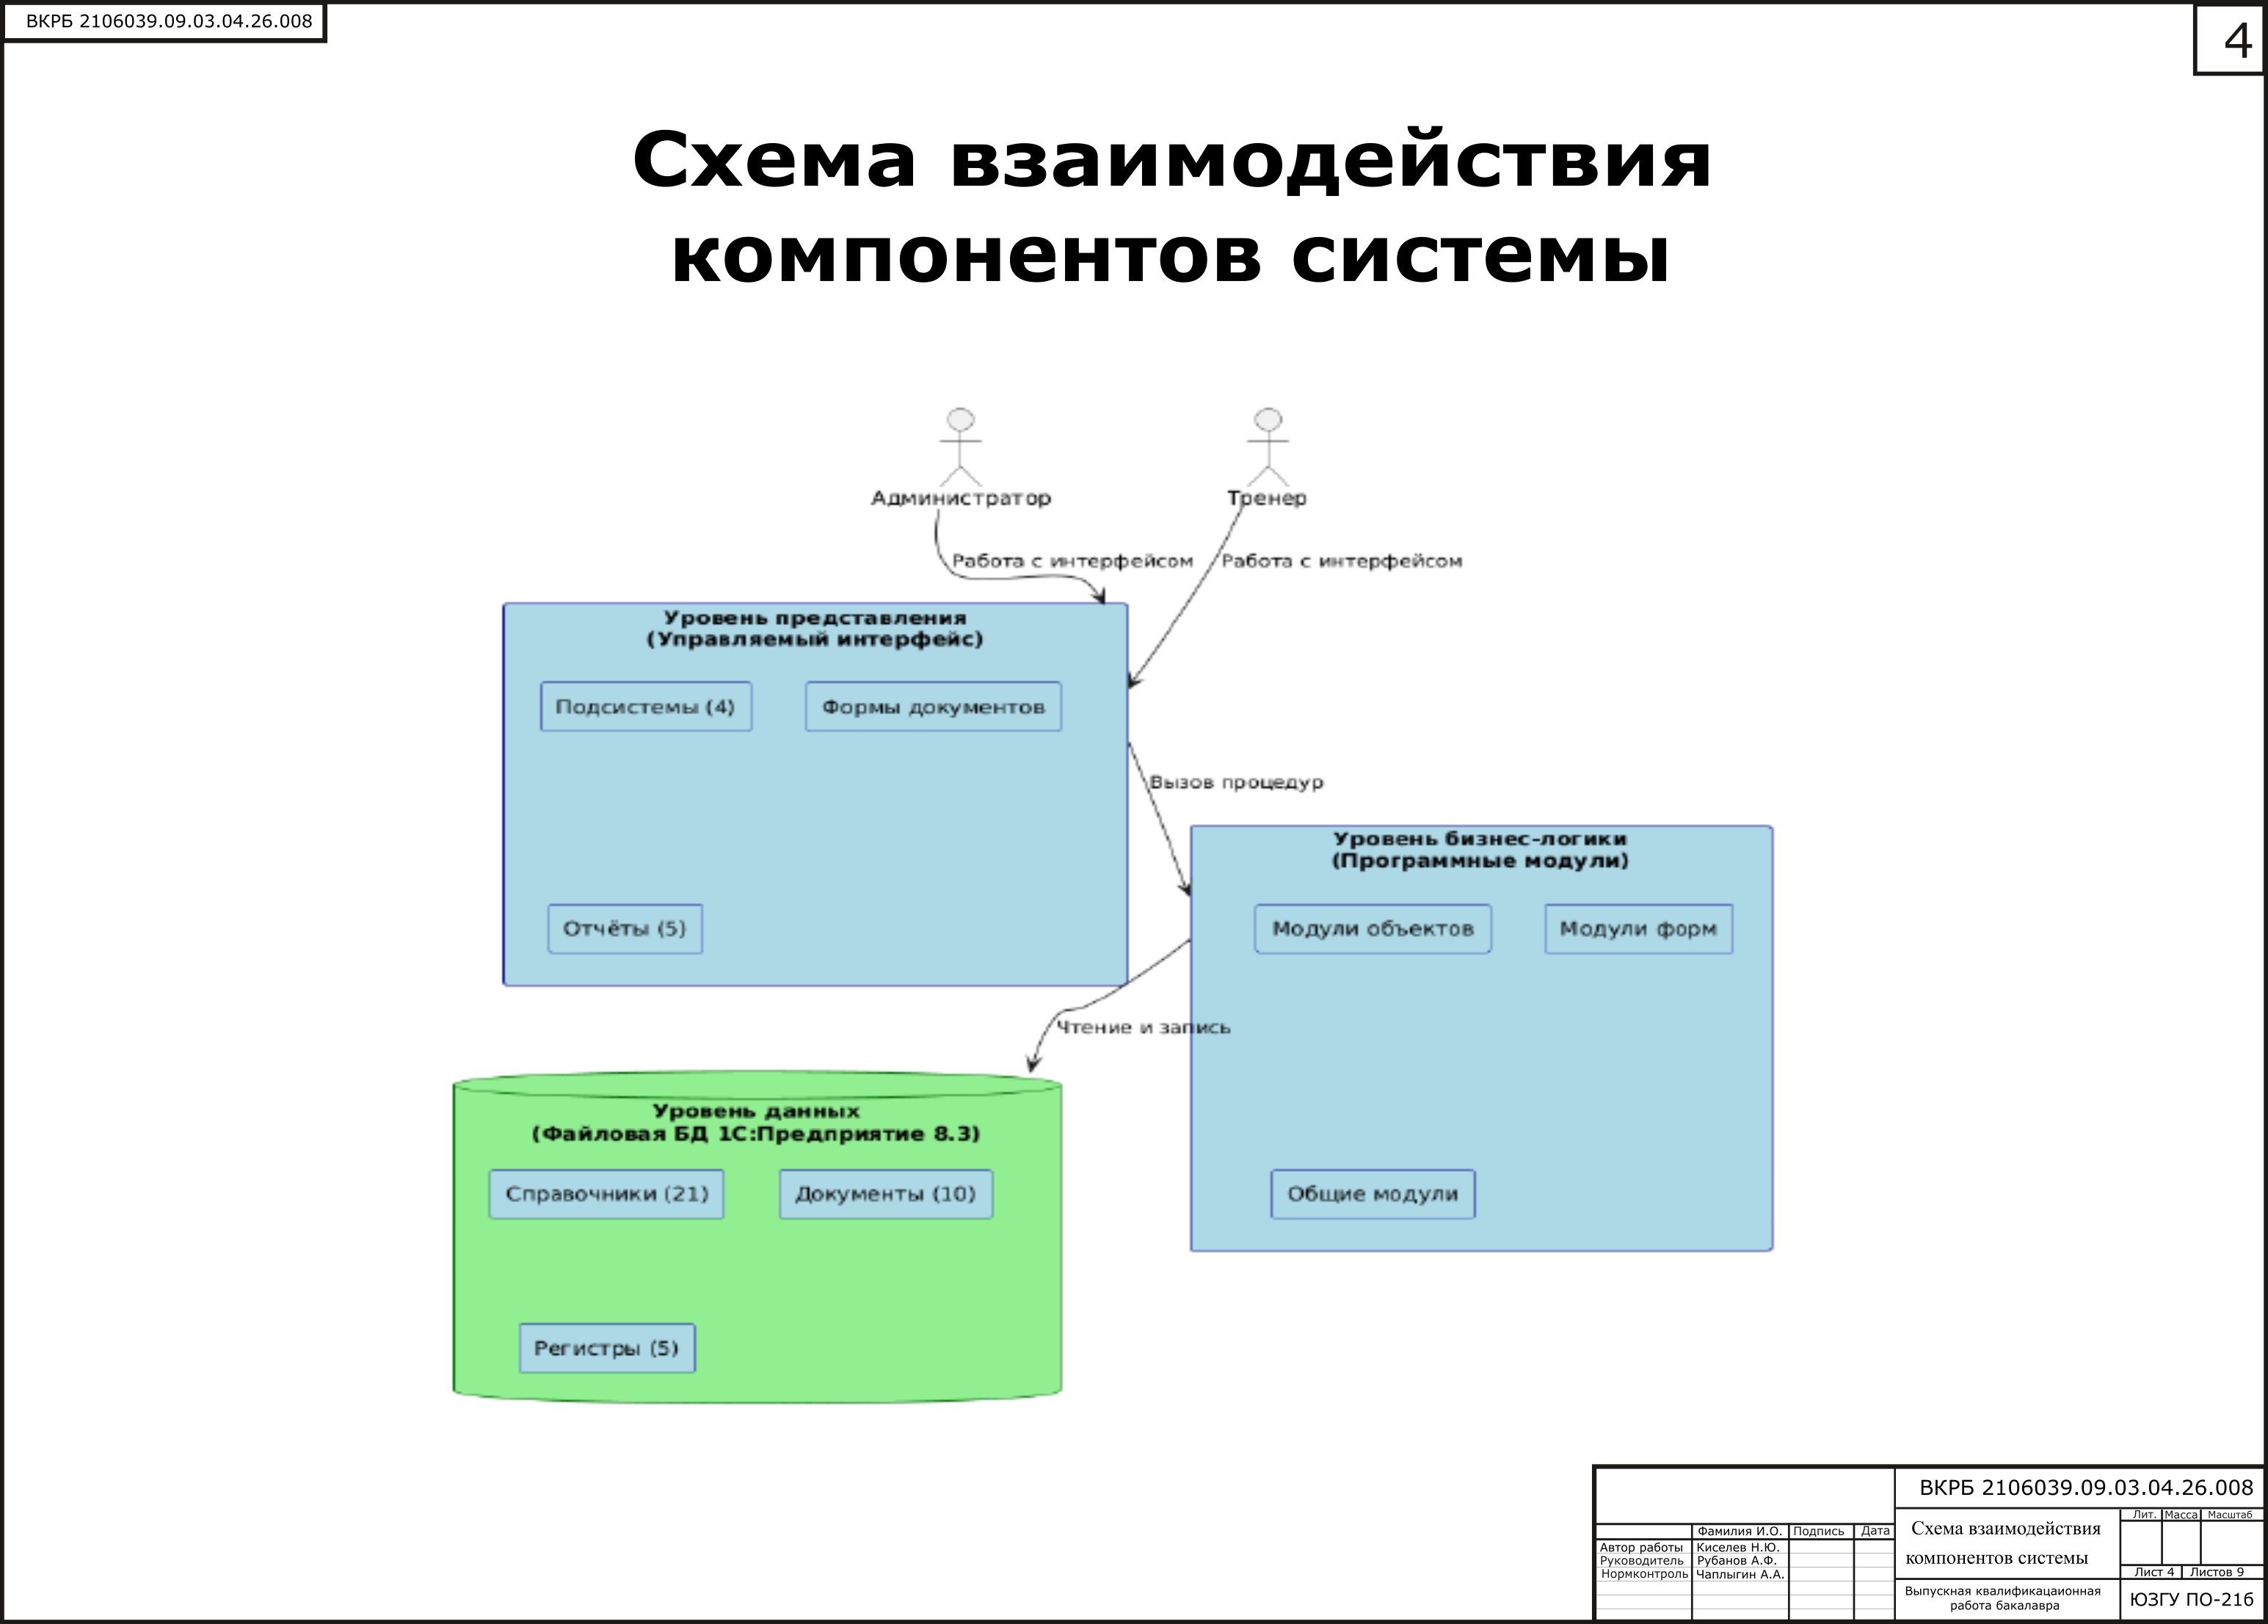
\includegraphics[width=0.85\linewidth]{images/Diplom4.png}
		\заголовок{Схема взаимодействия компонентов системы}
		\label{pl4:image}      
	\end{плакат}
	
	\begin{плакат}
		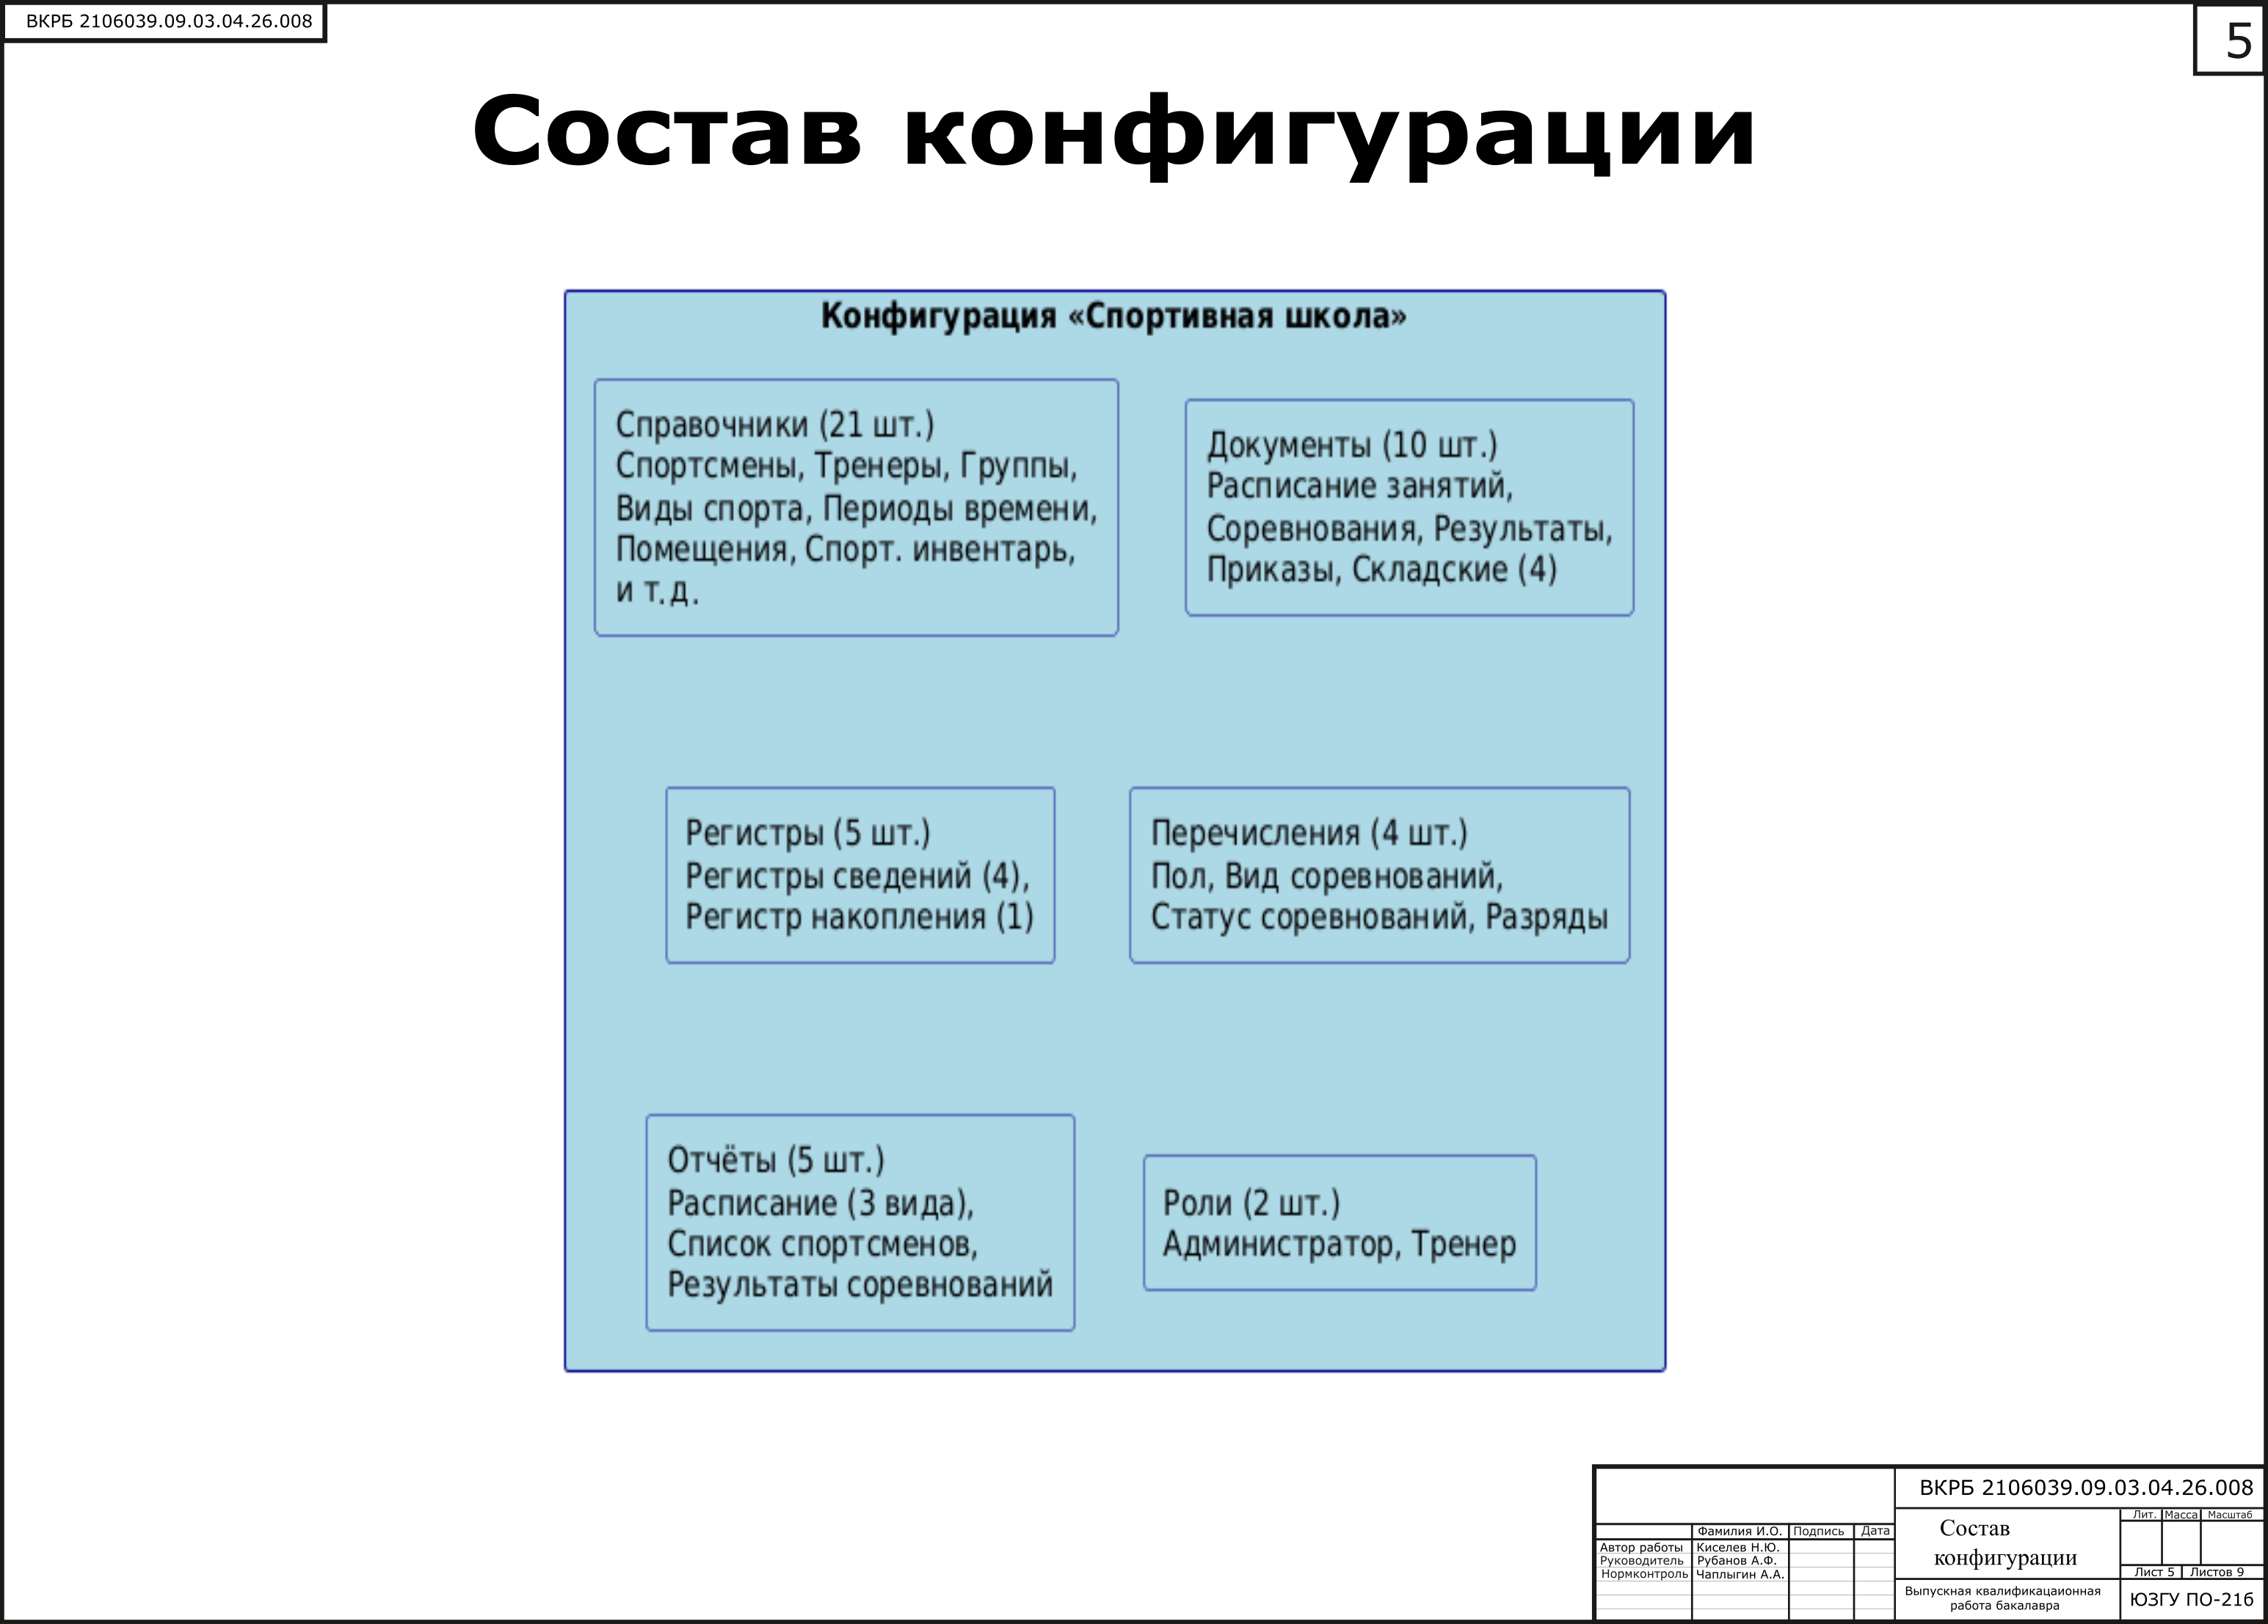
\includegraphics[width=0.85\linewidth]{images/Diplom5.png}
		\заголовок{Состав конфигурации}
		\label{pl5:image}      
	\end{плакат}
	
	\begin{плакат}
		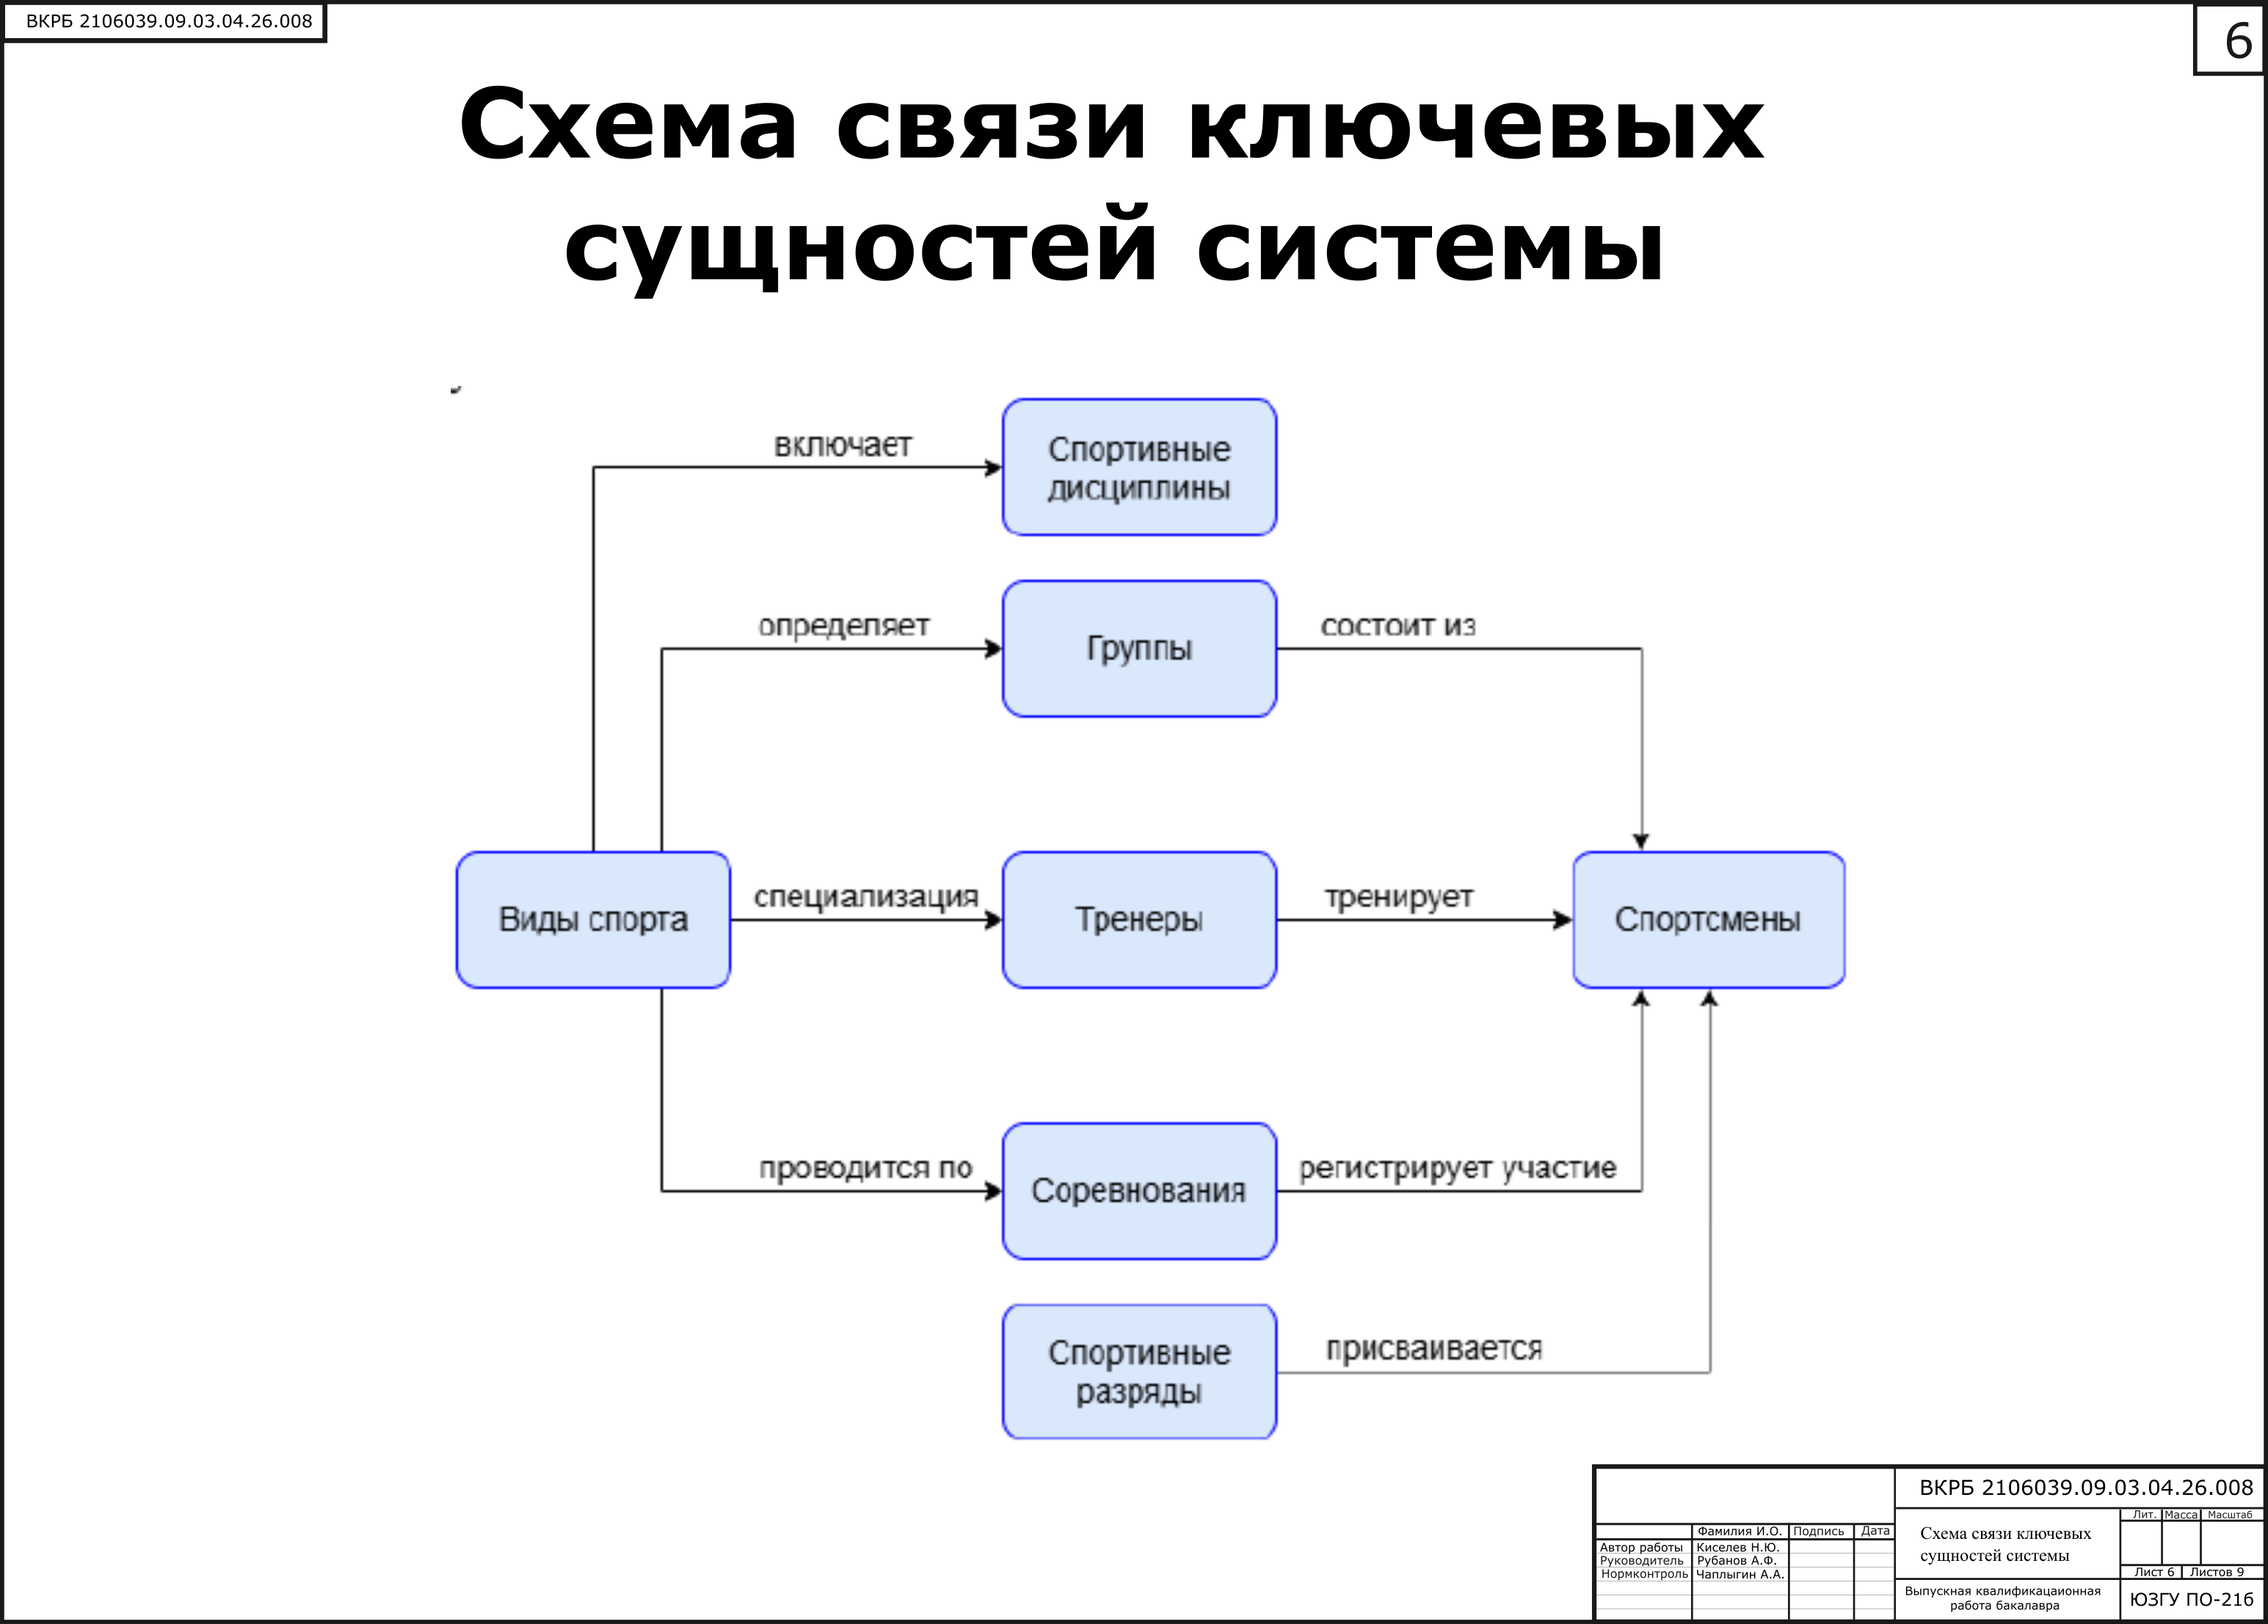
\includegraphics[width=0.85\linewidth]{images/Diplom6.png}
		\заголовок{Схема связи ключевых сущностей системы}
		\label{pl6:image}      
	\end{плакат}
	
	\begin{плакат}
		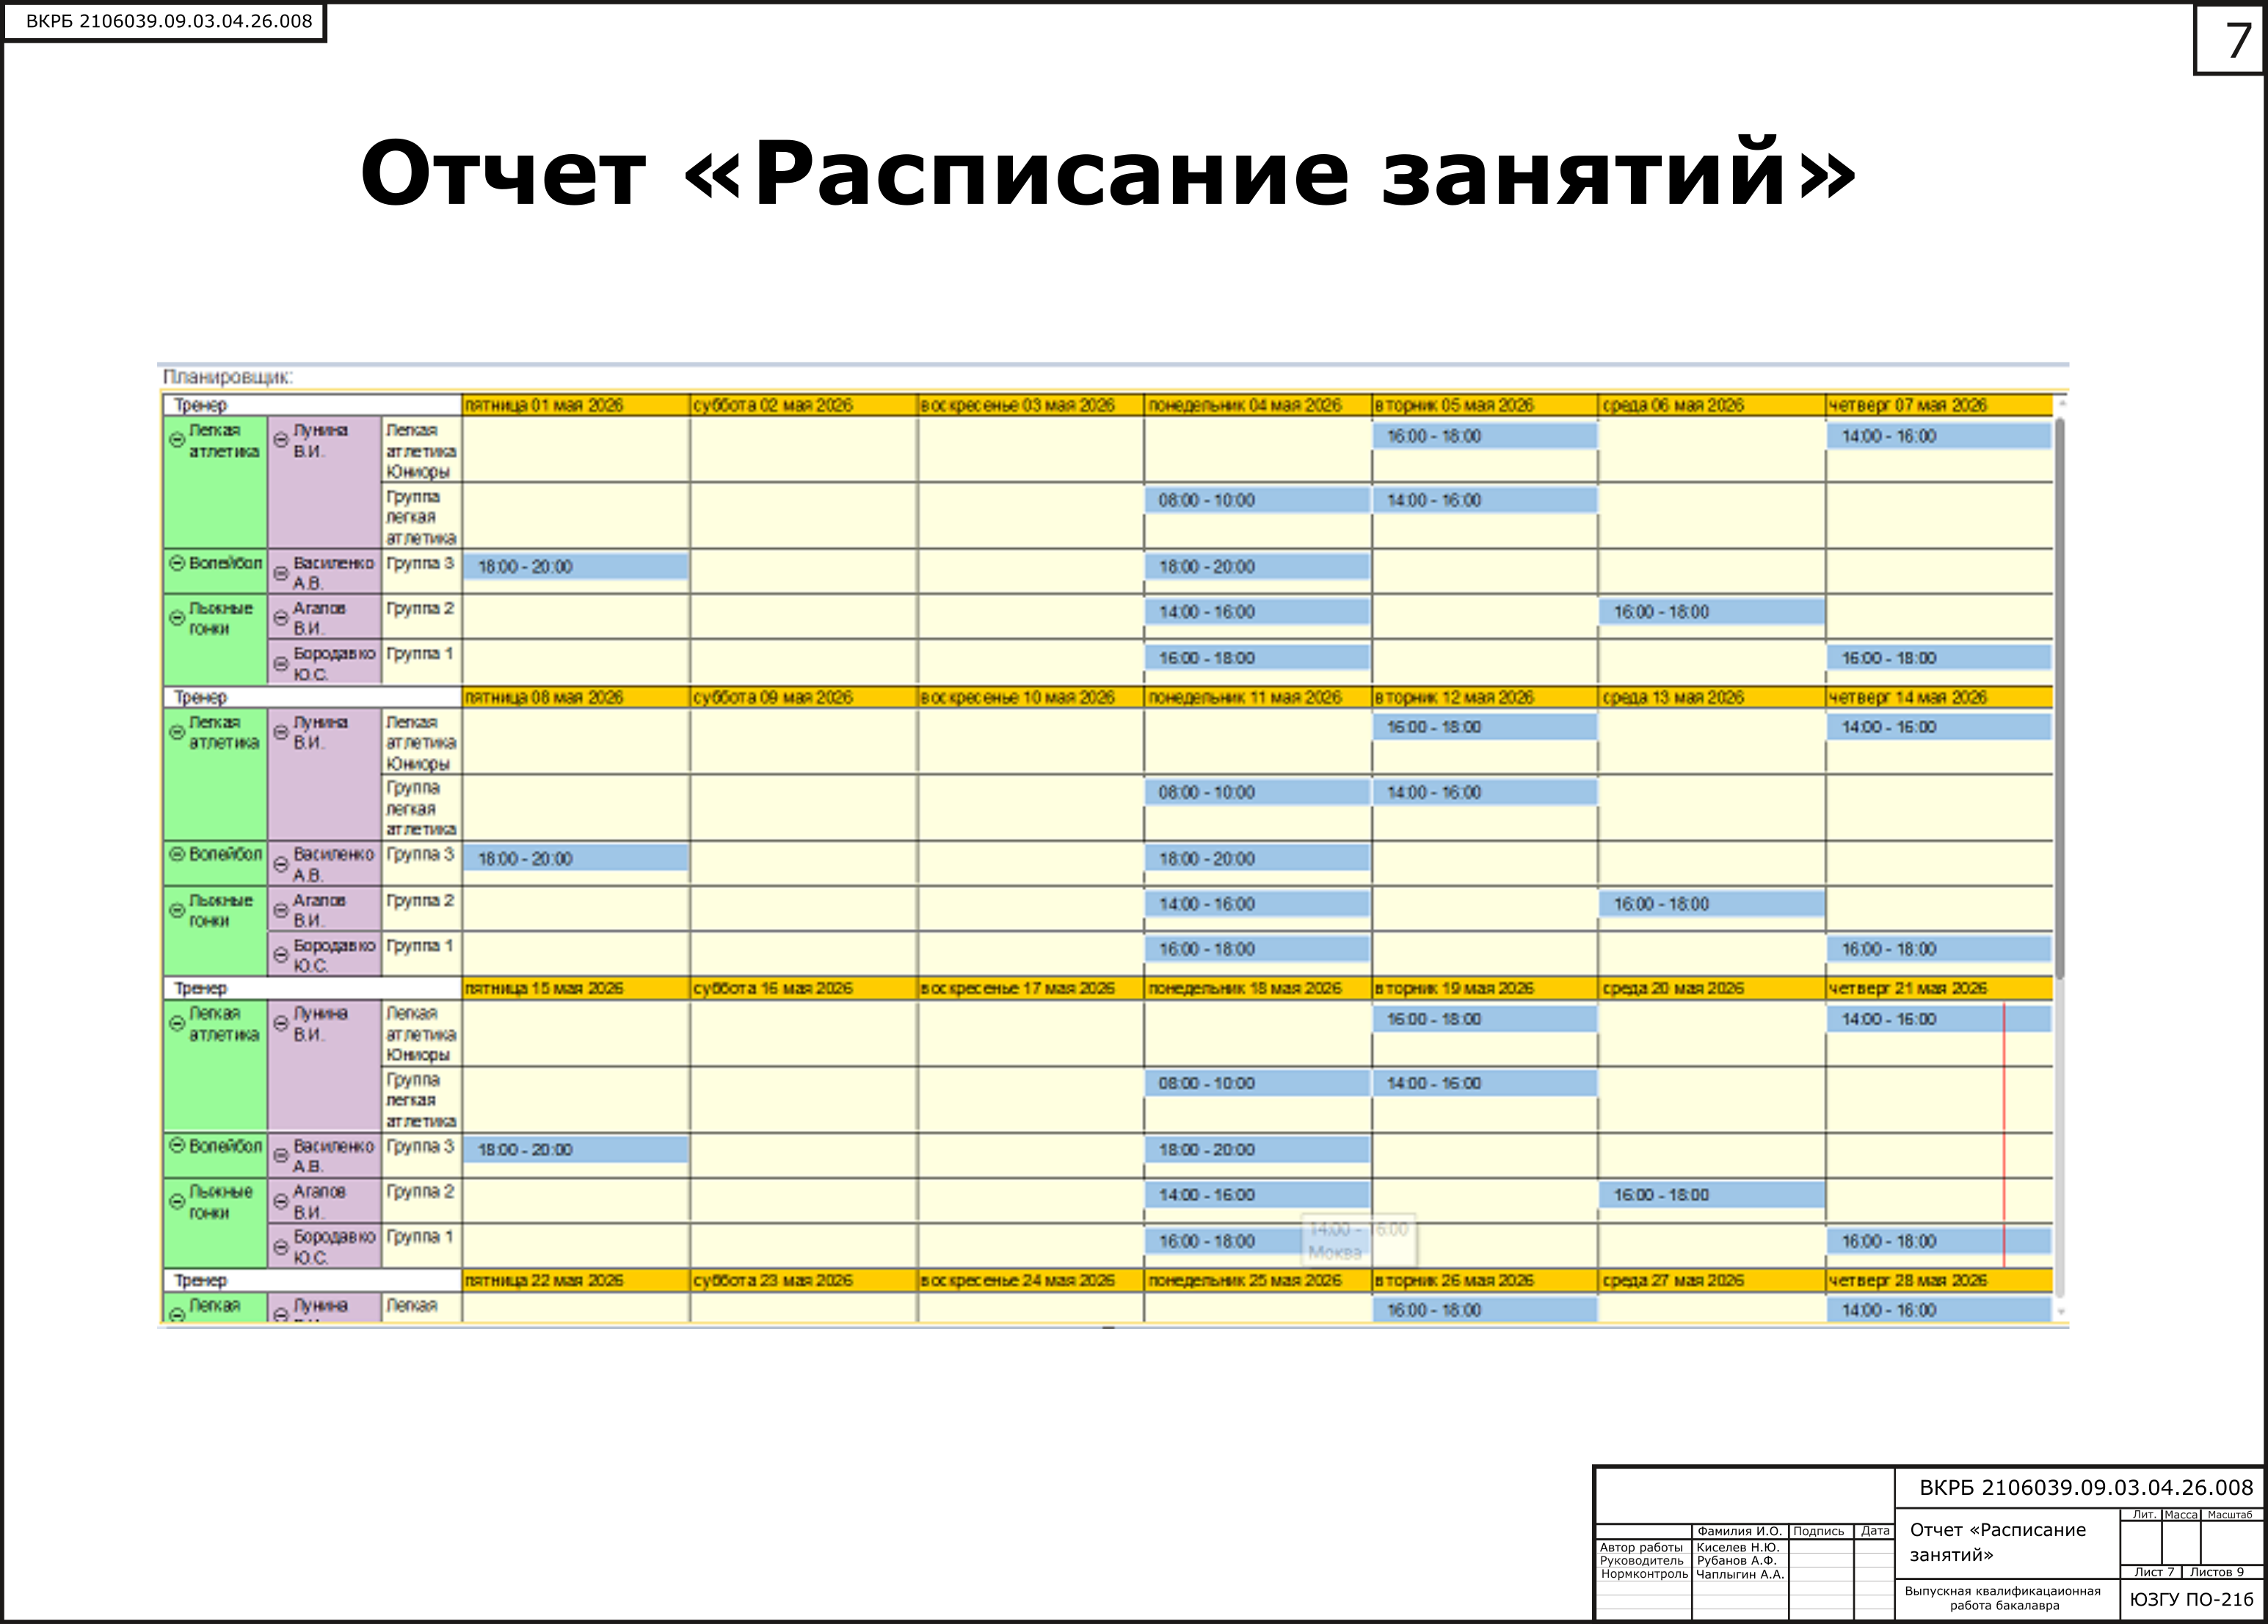
\includegraphics[width=0.85\linewidth]{images/Diplom7.png}
		\заголовок{Отчет «Расписание занятий»}
		\label{pl7:image}      
	\end{плакат}
	
	\begin{плакат}
		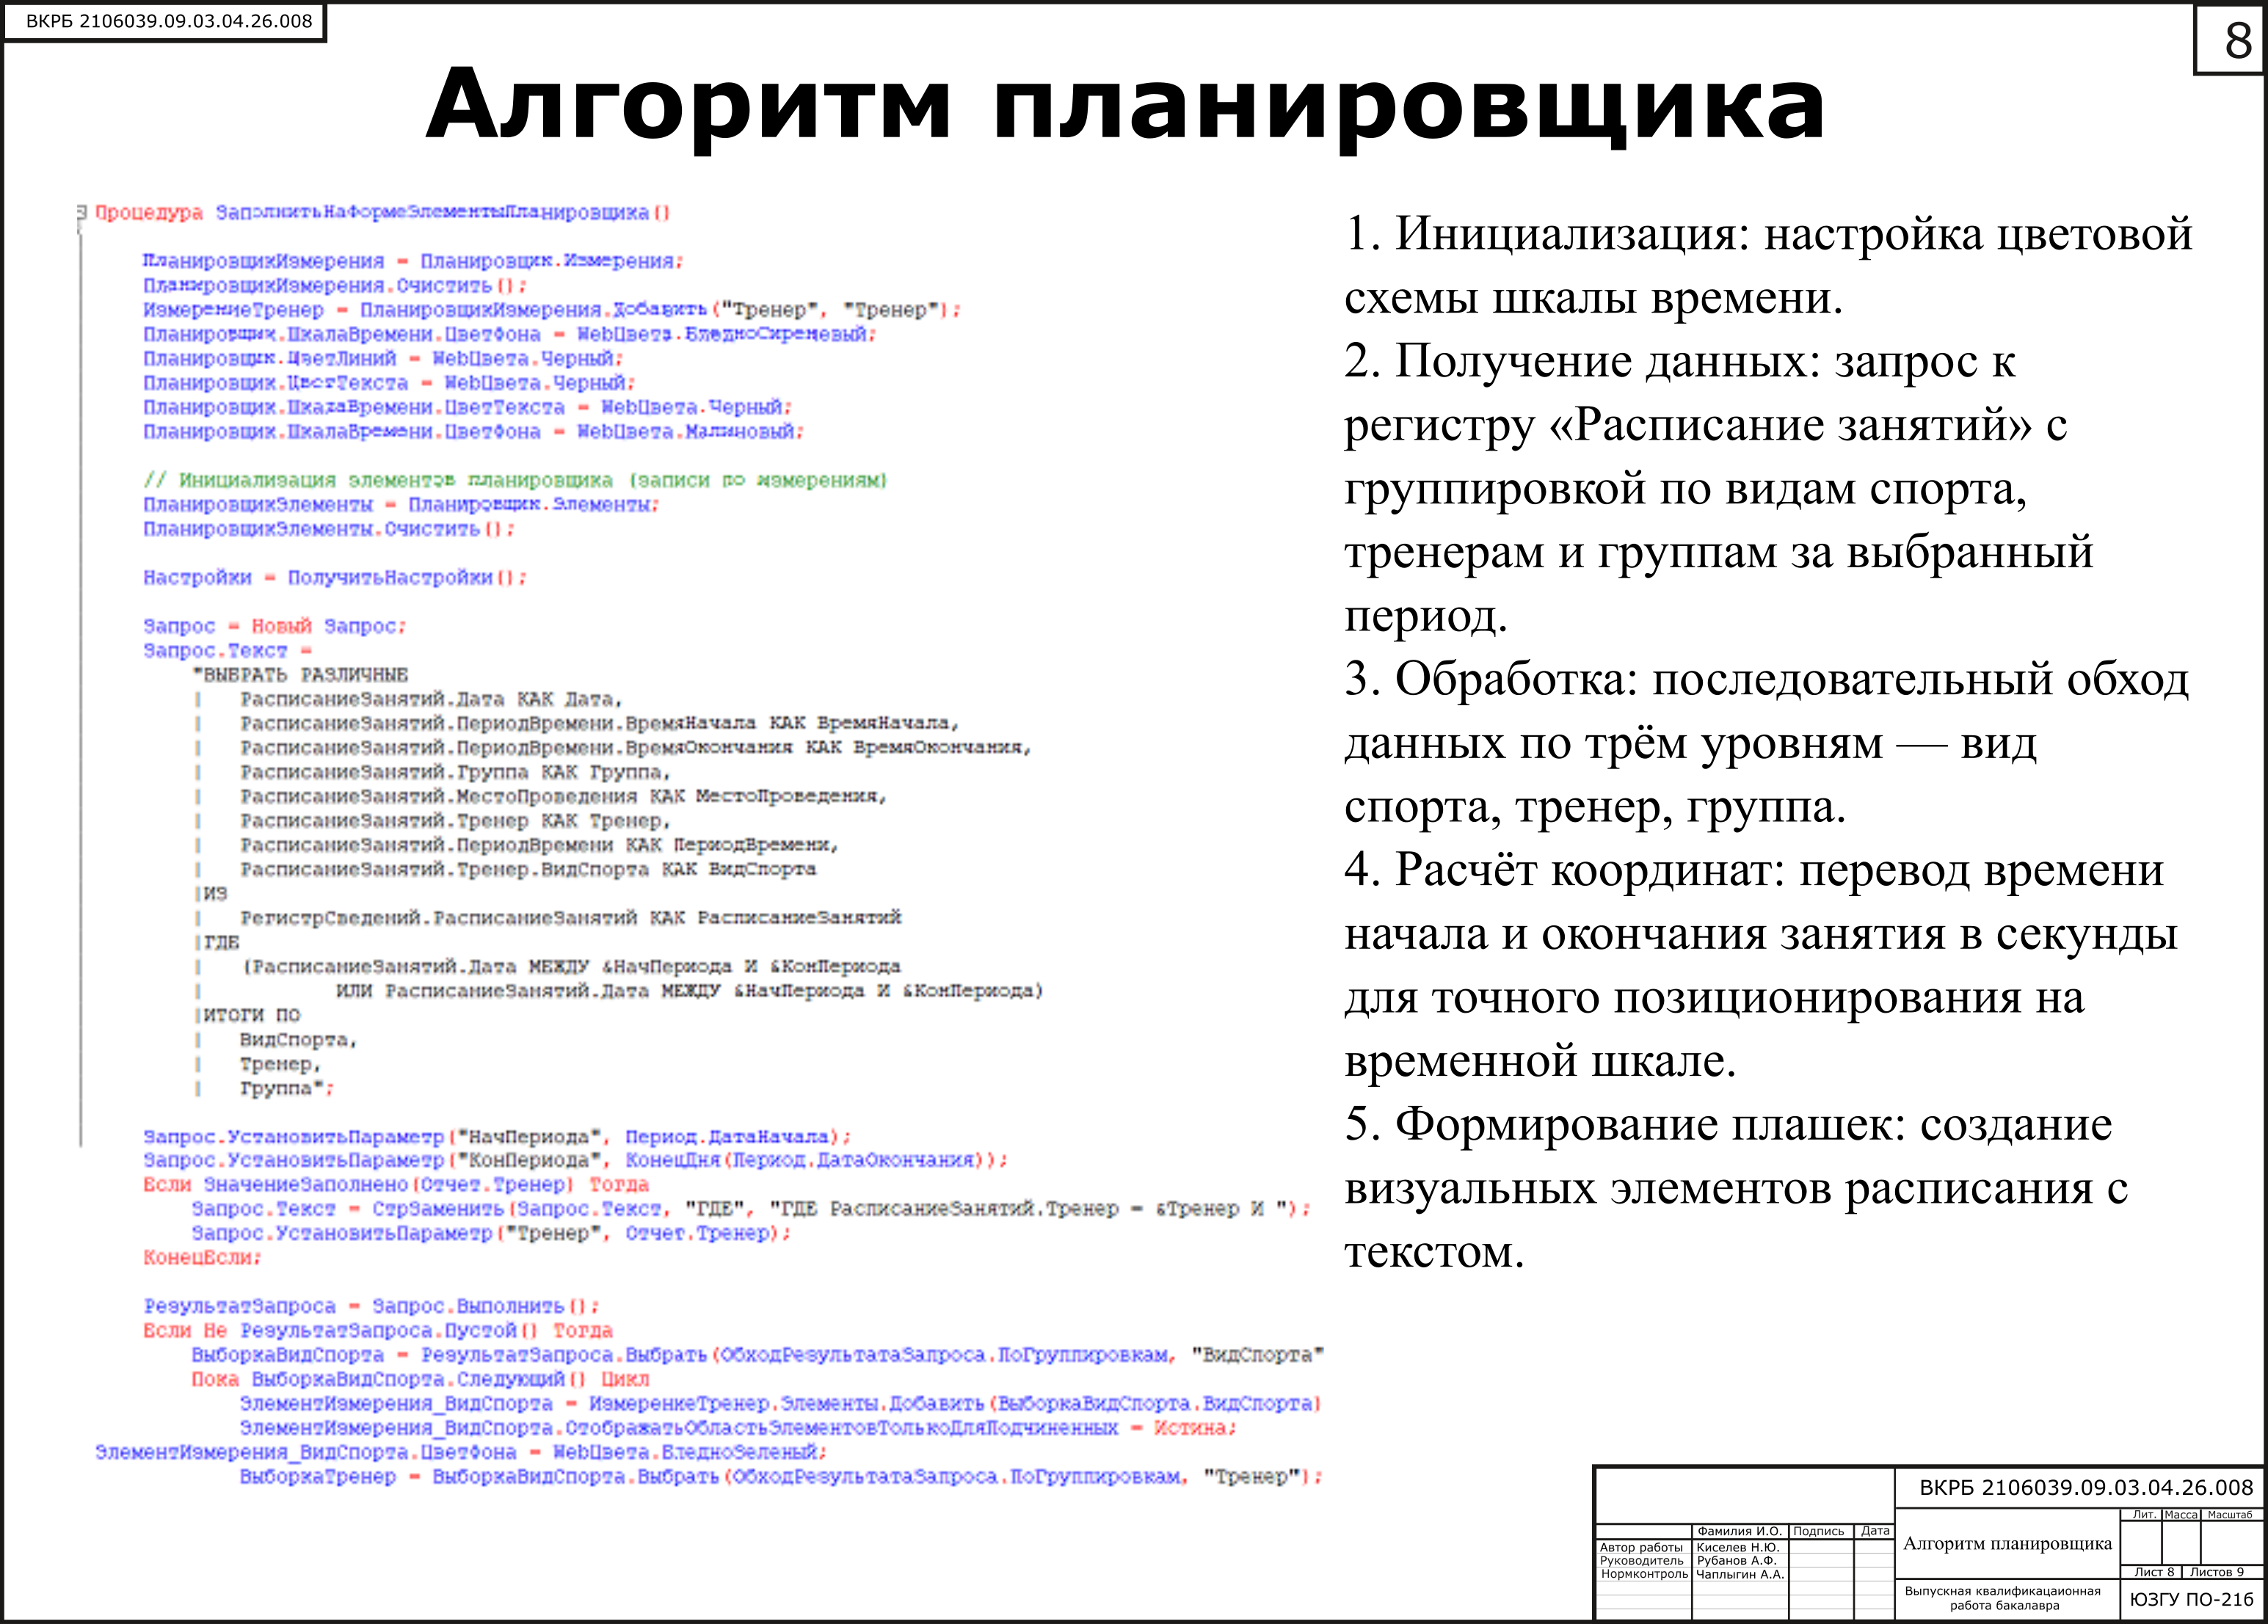
\includegraphics[width=0.85\linewidth]{images/Diplom8.png}
		\заголовок{Алгоритм планировщика}
		\label{pl8:image}      
	\end{плакат}
	
	\begin{плакат}
		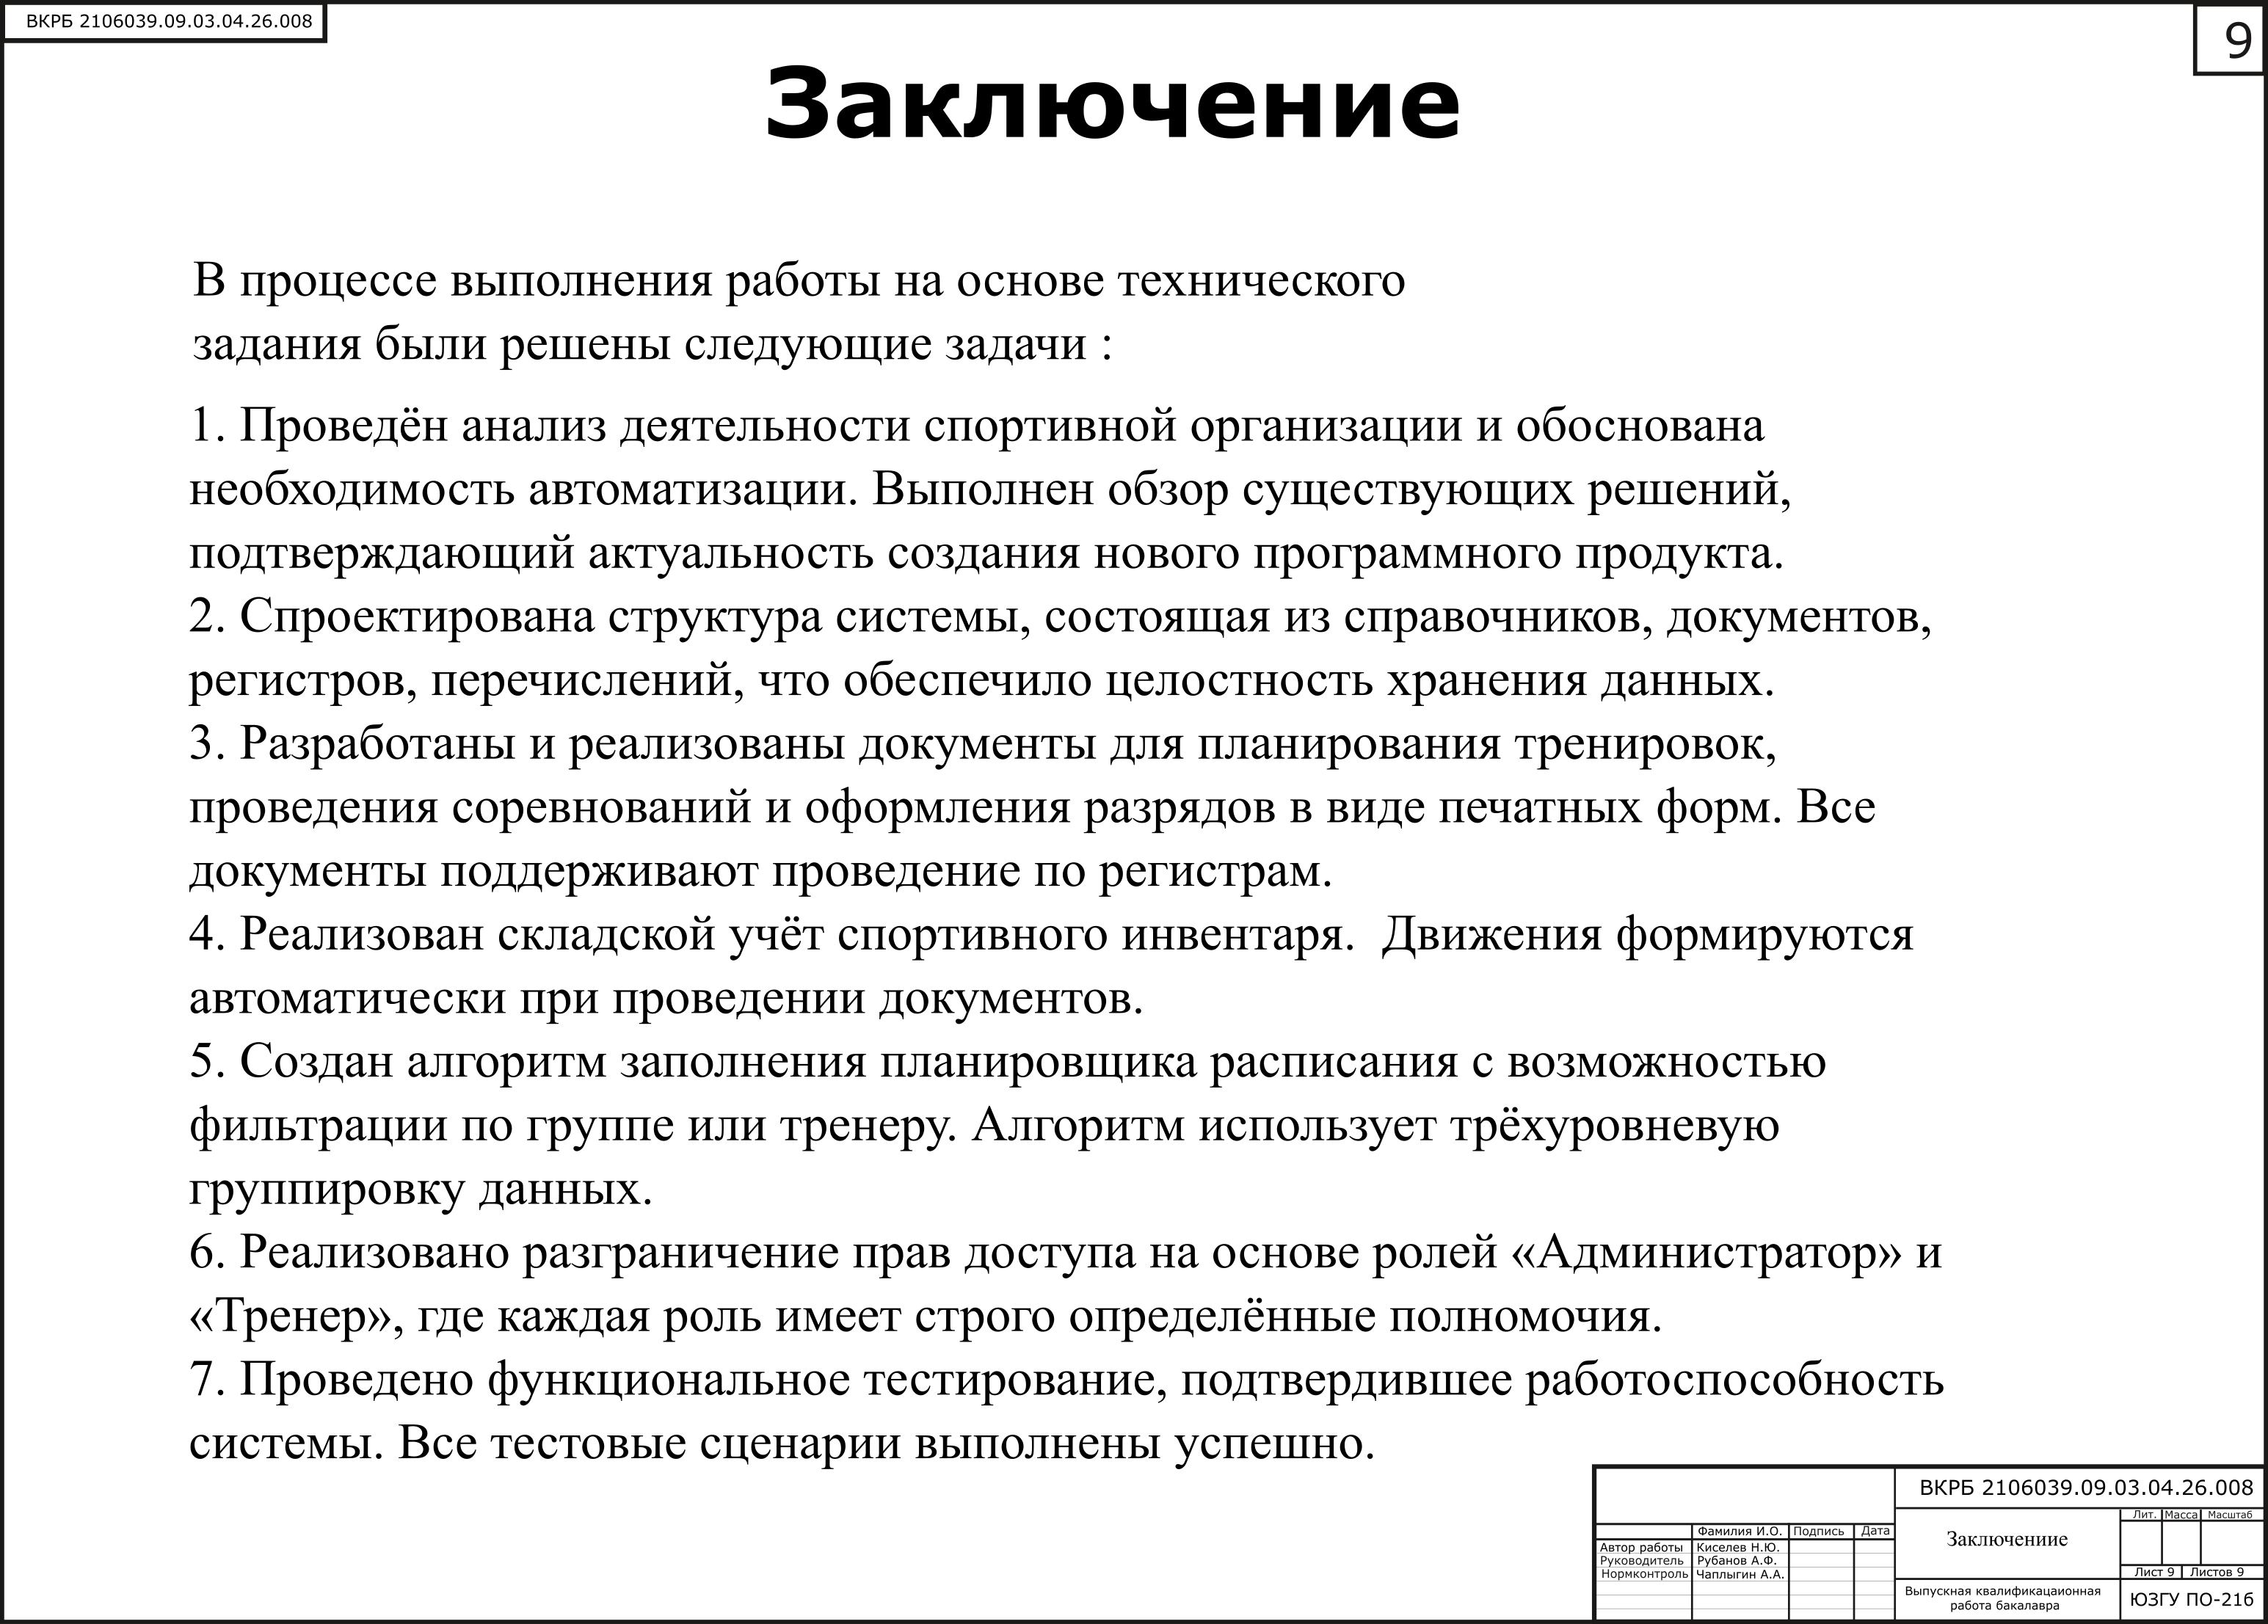
\includegraphics[width=0.85\linewidth]{images/Diplom9.png}
		\заголовок{Заключение}
		\label{pl9:image}      
	\end{плакат}
	
\end{landscape}
